\documentclass[a0]{sciposter}
\usepackage[width = 84.10cm, height = 118.90cm, left = 0cm, right = 2.12cm, top = 0cm, bottom = 0cm]{geometry}

\usepackage[english]{babel}
\usepackage[utf8]{inputenc}

\usepackage{graphicx}
\usepackage{ulem}

\usepackage{xcolor}
\definecolor{BoxCol}{HTML}{E5E5E5}
\definecolor{InfoBoxCol}{HTML}{F1A42B}
\definecolor{HeadCol}{HTML}{1E64C8}

\usepackage{multicol}
\setlength{\columnseprule}{0pt}
\setlength{\columnsep}{1.75cm}

\usepackage{qrcode}

\begin{document}
\vspace*{-2cm}\hspace*{-2cm}
\includegraphics[width = 14.47cm, height = 6.2cm]{img/logos/icon_UGent_LW_EN_RGB_2400_color.png}

\colorbox{BoxCol}{
\begin{minipage}[t][102cm][t]{82cm}

\vspace{2cm}\hspace{2cm}\begin{minipage}[t]{77cm}
{\fontsize{50}{52}\selectfont\textcolor{HeadCol}{\uppercase{BantUGent - UGent Centre for Bantu Studies}}}
\bigbreak\bigbreak
{\fontsize{40}{44}\selectfont{\textbf{Dirk Seidensticker\textsuperscript{1}, Bernard Clist\textsuperscript{1}, Wannes Hubau\textsuperscript{2}, Hans Beeckman\textsuperscript{2}, Sara Pacchiarotti\textsuperscript{1}, and Koen Bostoen\textsuperscript{1}}}}
\bigbreak\bigbreak
{\fontsize{44}{50}\selectfont\textcolor{HeadCol}{\uline{\textbf{\uppercase{The Late Holocene Settlement History of the Central African Rainforest:}}}}}
\bigbreak
{\fontsize{44}{50}\selectfont\textcolor{HeadCol}{\uline{\textbf{\uppercase{Archaeological, Palaeoenvironmental and Linguistic Evidence for 3,000 years of}}}}}
\bigbreak
{\fontsize{44}{50}\selectfont\textcolor{HeadCol}{\uline{\textbf{\uppercase{Interaction between Bantu Speech Communities and their Changing Environments}}}}}
\end{minipage}

\vspace{2cm}\hspace{2cm}\begin{minipage}[t]{77cm} %24.5cm
{\fontsize{28}{36} \selectfont During the past forty years, archaeological, palaeoenvironmental and linguistic research in the Central African rainforest have made a significant contribution to our understanding of the settlement history of one of Africa's major biotopes. Taking into account the massive extent of this biotope, the promising results of past research, which filled the blank spot that the rainforest represented on any archaeological distribution map of Africa until the 1970s, can only be seen as starting points. Our poster aims at reviewing our current state of knowledge on the settlement history of the Central African rainforest as documented within surveys and excavations as well as through the late Holocene palaeoenvironmental record between present-day Cameroon and Angola. The earliest traces of sedentary and potentially food producing people, mainly identified through pottery finds, date back to the first millennium BC and are commonly seen in relation to a contemporaneous crisis of the rainforest and to the expansion of Bantu languages.}
\end{minipage}

\vspace{1cm}
\hspace{2cm}\begin{minipage}[t]{77cm}
\begin{multicols}{3}

{\fontsize{38}{42} \selectfont \textcolor{HeadCol}{Archaeology}}
\bigbreak
{\fontsize{28}{36} \selectfont In the putative Bantu homeland in the Cameroonian Grassfields, archaeological research has shown that pottery of a specific style coexisted with a macrolithic toolkit from around 7,000~BP until 4,000~BP. A new and distinctive kind of pottery, similar to the earlier Grassfields ones and associated with the region now covered by rainforest, develops only after 3,000~BP in southern Cameroon. The spread of these early groups further south show a general north to south chronological gradient reaching the Inner Congo Basin and the Lower Congo around 2,400--2,300~BP. Metallurgy is rare then but becomes more abundant after 2,000~BP.}
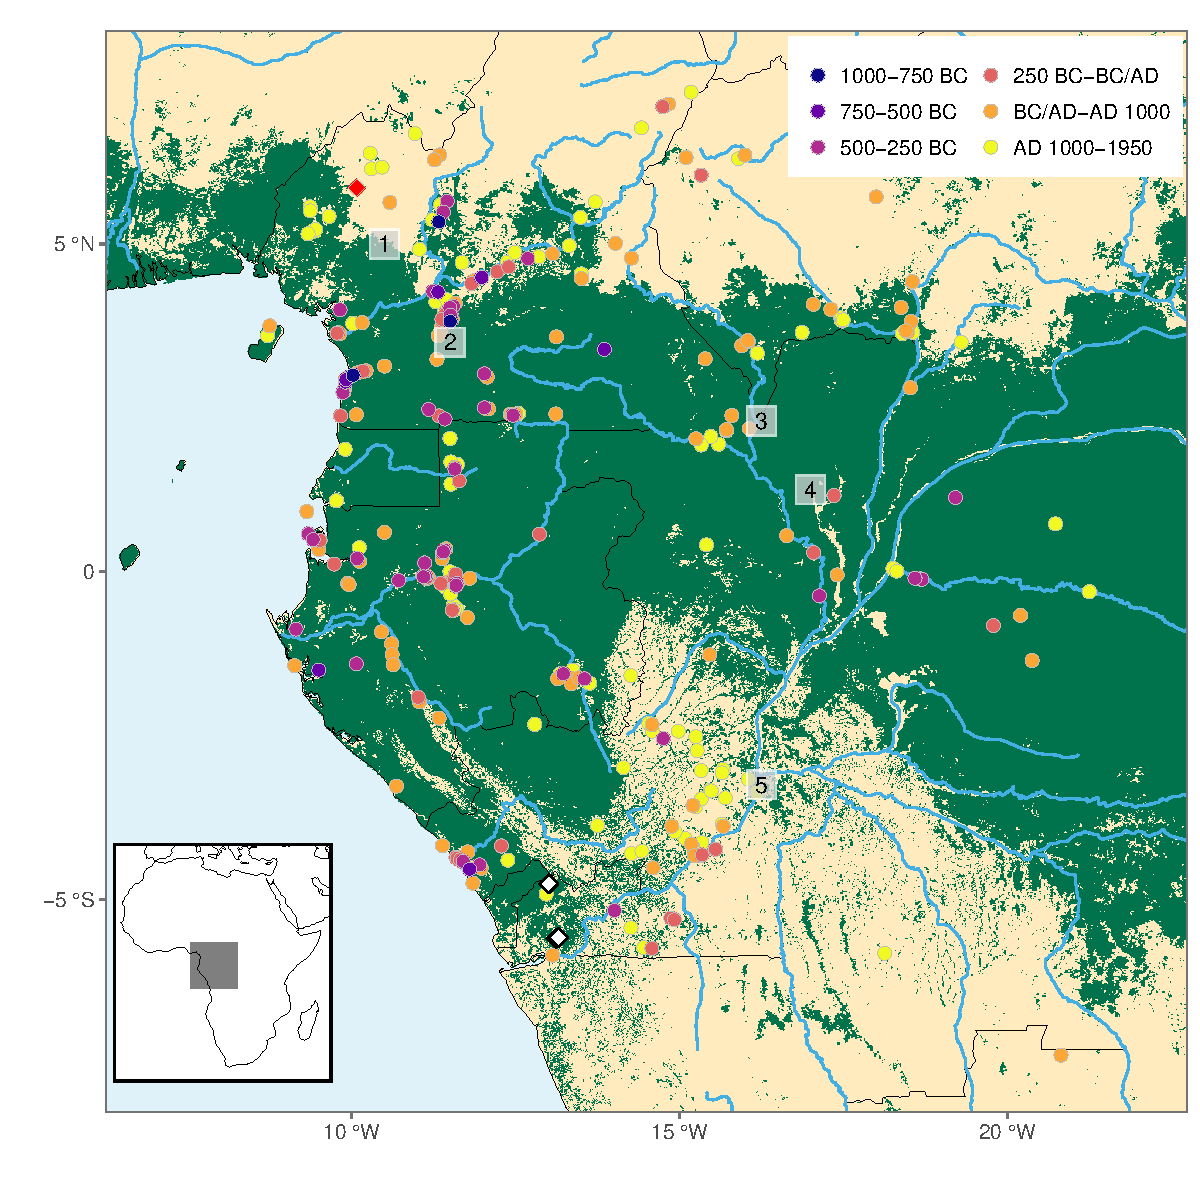
\includegraphics[width = \linewidth]{img/FigArch-A_map.pdf}
{\fontsize{22}{0} \selectfont \textit{\textbf{Fig.~1}\hspace{1em}Mapping of dated archaeological sites from the last 3000 years. White diamonds: Palaeoenvironmental sites (see \textbf{Fig. 2}). Numbers: Successive hubs of Bantu language dispersal (see \textbf{Fig. 3}).}}
\bigbreak
{\fontsize{28}{36} \selectfont Empirical evidence of past subsistence is rare. Isolated finds associated with the earliest traces of pottery producing groups indicate a mixed system consisting of hunting, collecting, fishing, small stock raising, and horticulture. The questions of what constituted the subsistence base of those early sedentary groups and if this was a package carried into the forests, or developed as successive adaptations is still debated.}
\bigbreak
{\fontsize{28}{36} \selectfont A comparison of the archaeological record of the western/coastal area, characterized by a diverse history of research, and the Congo Basin, whose archaeological record goes back to the River Reconnaissance Project (1977--1987), indicates separate migration axes. The oldest evidence for pottery-producing settlers north and south of the Congo mouth, within the present-day confines of the so-called \textit{West-Coastal} Bantu languages (\textbf{Fig. 3}), date between 2,700--2,350~BP (Loango coast) and 2,300--2,000 BP (Lower Congo) respectively. Changes in pottery styles and technology along the Atlantic as well as the tributaries of the Congo River are probably indicative of multiple small-scale immigration movements.}
\vfill\null
\columnbreak
{\fontsize{38}{42} \selectfont \textcolor{HeadCol}{Palaeoecology}}
\bigbreak
{\fontsize{28}{36} \selectfont Palaeoenvironmental evidence shows that climatic anomalies had an impact on Central African vegetation. Intense droughts are thought to have left the forest structure severely fragmented. This happened especially during the third millennium BP rainforest crisis (3,000--2,000 BP). The period is characterized by increasing sea surface temperatures (SST) near the Congo River mouth. Peaks in SST are associated with drought periods on the Central African continent. During these periods, contiguous forest areas were turned into mosaics of forest and savanna patches.}
\bigbreak
\colorbox{white}{\includegraphics[width = \linewidth, height=1.1\linewidth]{img/"Hubau et al 2015 GCB timeline".pdf}}
\bigbreak
{\fontsize{22}{0} \selectfont \textit{\textbf{Fig.~2}\hspace{1em}Charcoal identification results from 6 pits excavated in the Mayumbe rainforest (see \textbf{Fig.~1}). Each box represents a pit and each colored histogram a charcoal assemblage formed during a fire event. The classification represents ecological preferences of the identified taxa. Identification of radiocarbon dated charcoal fragments shows that pioneer (light green) and woodland savanna taxa (brown) were sometimes still dominant in charcoal assemblages that were formed centuries after the actual disturbance periods (gray areas). This suggests that forest regeneration after intense drought periods may have been a slow process, hampered by recurring fire events. Open savanna patches remained fire-prone even after the drought anomalies, and savanna fires may have impacted nearby forest edges and hampered forest encroachment (Source: Hubau et al. 2015).}}
\bigbreak
{\fontsize{28}{36} \selectfont Although climate-driven forest disturbance certainly occurred during drought periods throughout the Holocene, migrating Bantu speaking villagers may have locally reinforced the process of forest destruction by applying slash-and burn techniques in rainforest areas. However, human impact was probably more important during the last millennium. It is still unclear how significant anthropogenic factors were during the third millennium BP rainforest crisis.}
\vfill\null
\columnbreak
{\fontsize{38}{42} \selectfont \textcolor{HeadCol}{Linguistics}}
\bigbreak
{\fontsize{28}{36} \selectfont Within the Bantu area, the North-West, more specifically Cameroon and northern Gabon, is linguistically the most heterogeneous. This high linguistic diversity suggests that the earliest phases of the Bantu Expansion were characterized by slow and small-scale language dispersal. The rest of the Bantu area is occupied by four major branches, which emerged after the initial diversification. Three of them consist of languages spoken in the western half of the Bantu domain: (1) \textit{Central-Western}/\textit{North Zaire}/\textit{Congo}, (2) \textit{West-Coastal}/\textit{West-Western} and (3) \textit{South-Western}. All Bantu languages spoken in Eastern and South-Eastern Africa belong to a single \textit{Eastern} branch.}
\bigbreak
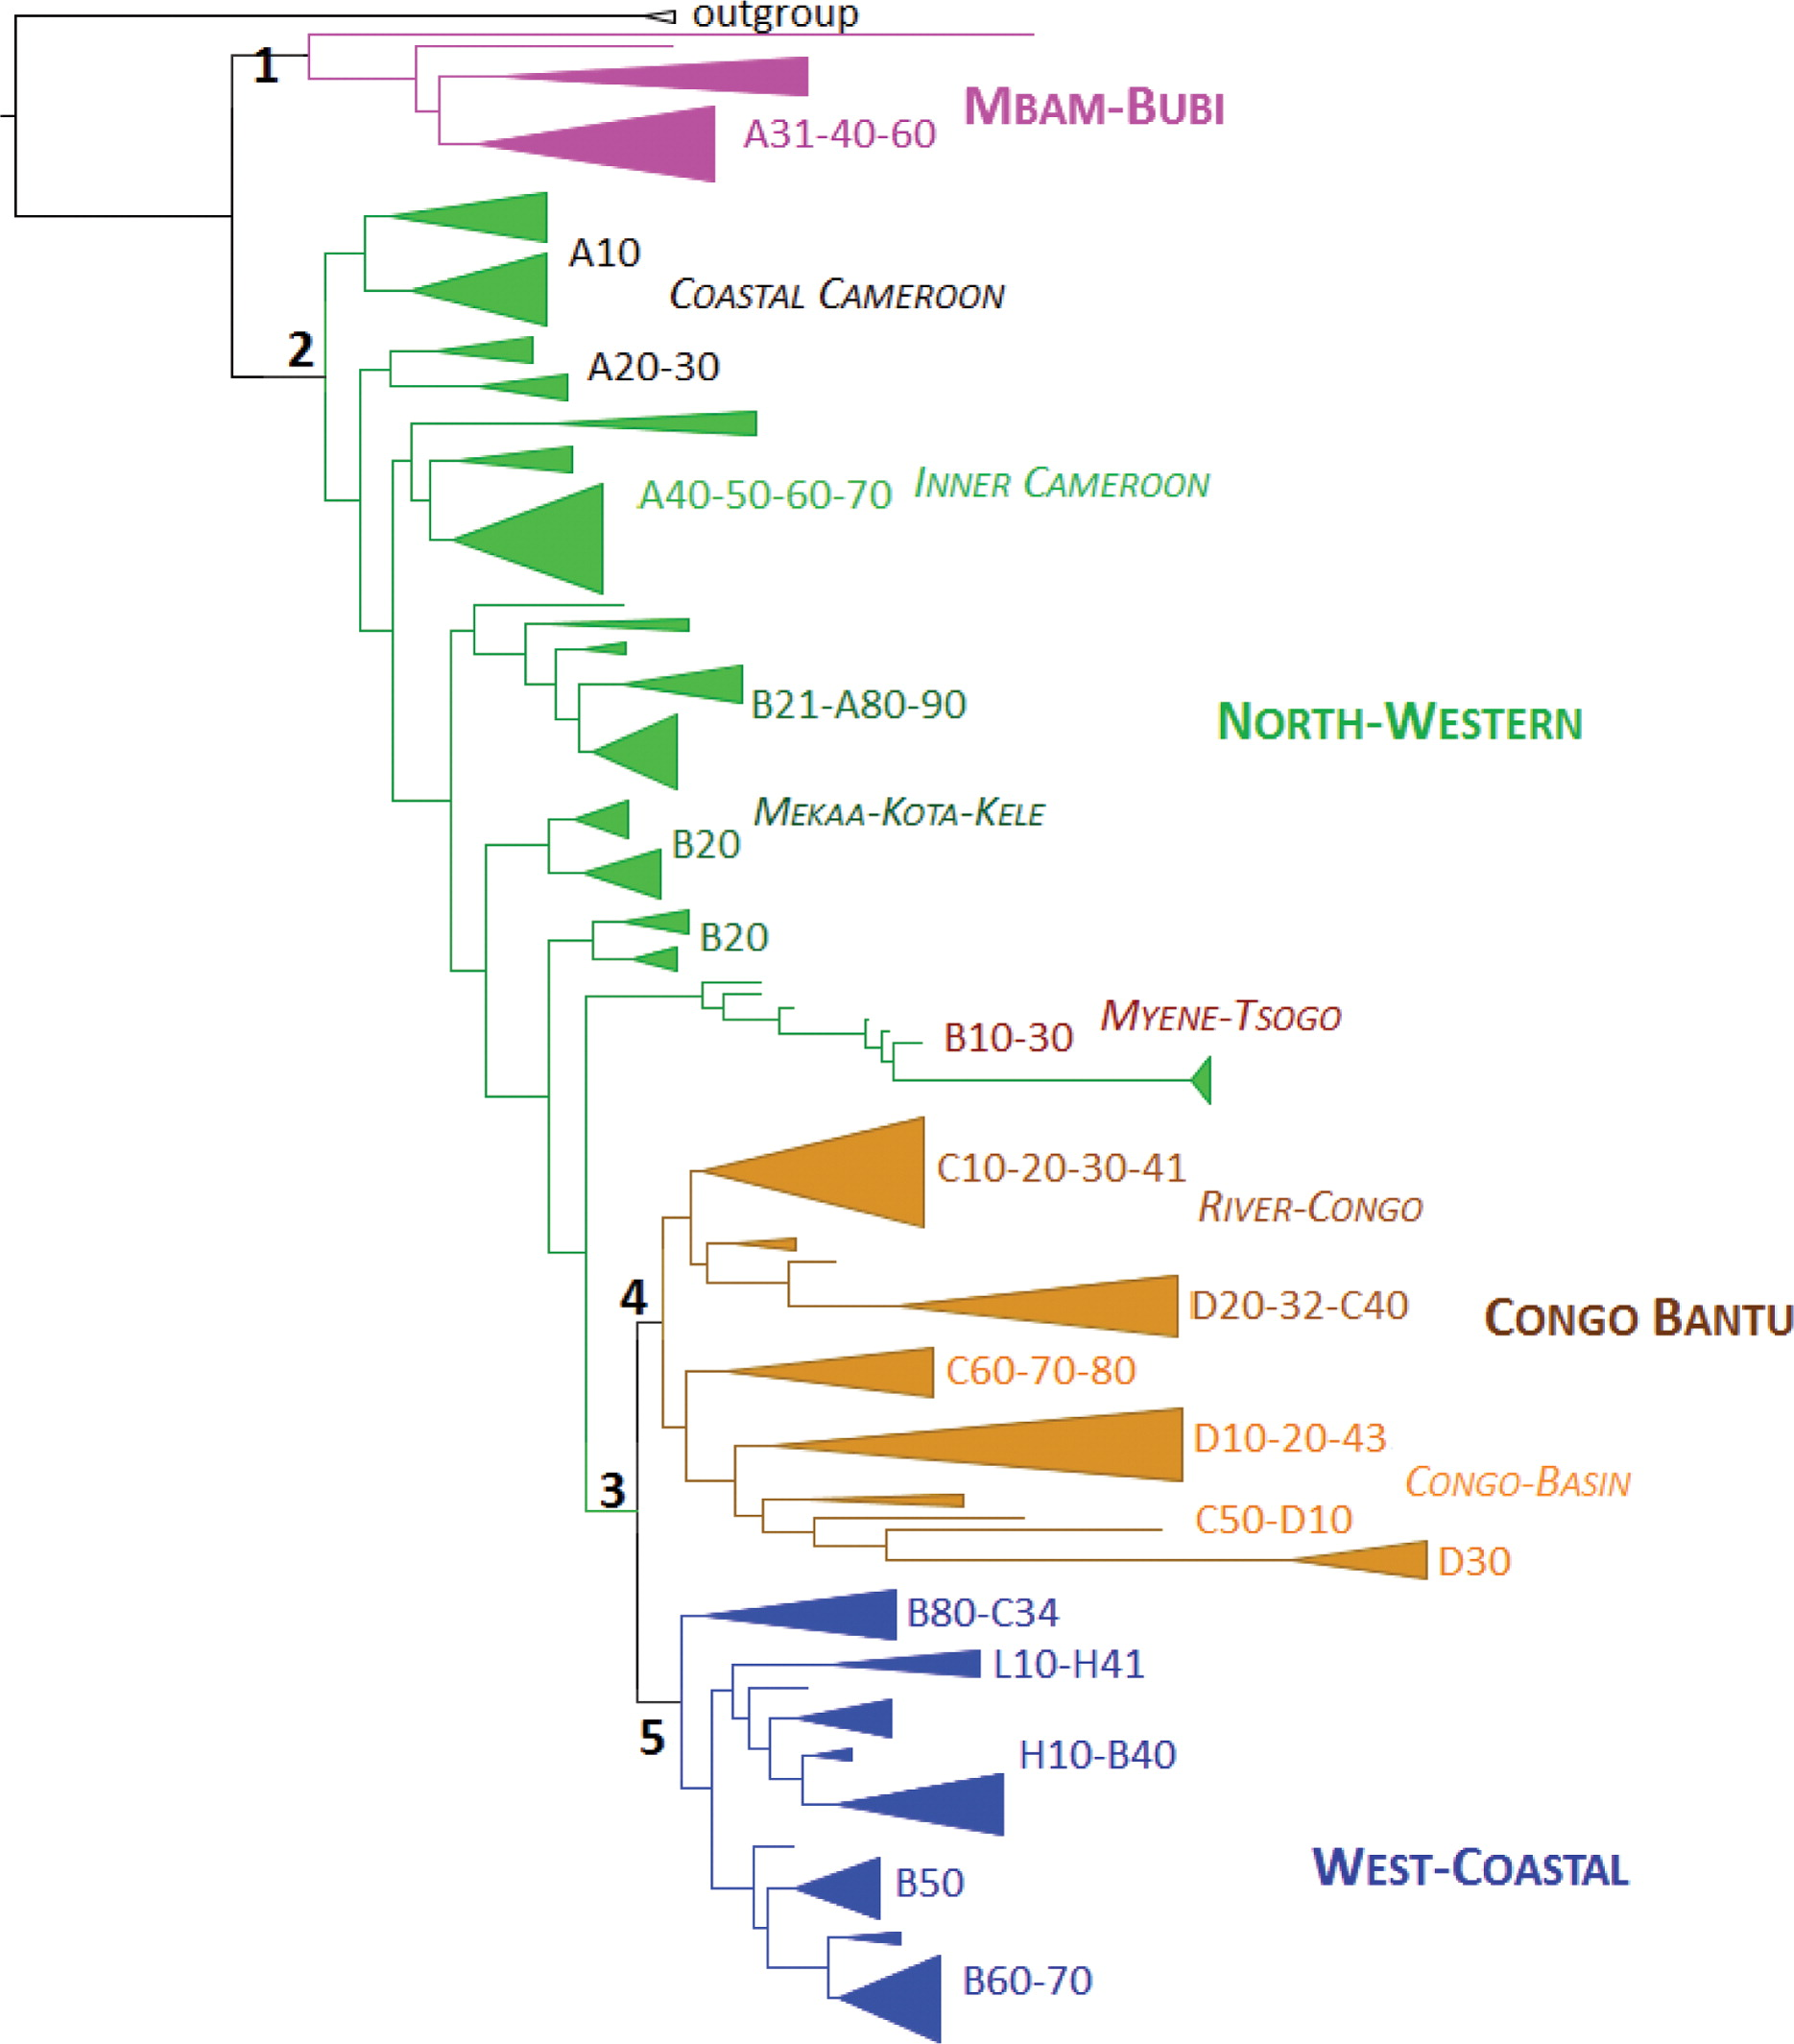
\includegraphics[width = \linewidth, height=1.125\linewidth]{img/fg3_online.jpeg}
\bigbreak
{\fontsize{22}{0} \selectfont \textit{\textbf{Fig.~3}\hspace{1em}Simplified Bayesian consensus tree of 168 Bantu languages. Numbers on the tree correspond to successive hubs of Bantu language dispersal (see \textbf{Fig.~1}; Source: Bostoen et al. 2015).}}
\bigbreak
{\fontsize{28}{36} \selectfont Grollemund et al. 2015 and de Schryver et al. (2015) show that \textit{West-Coastal} Bantu is composed of three distinct subclades: the \textit{Kikongo Language Cluster} (KLC), the \textit{Yanzi} languages and the \textit{Nzebi-Mbete-Teke} languages. The putative homeland of these three subgroups would be situated somewhere in between the Bateke Plateau and the Bandundu region of Congo DRC (2--4$^\circ$S/14--17$^\circ$E) and would not have emerged before ca. 2,500 BP. While the ancestors of \textit{Nzebi-Mbete-Teke} languages remained relatively close to the putative \textit{West-Coastal} homeland, the ancestors of Yanzi speakers must have moved east of the Congo River and KLC speakers must have moved towards the Atlantic Ocean instead. Following Grollemund et al. (2015), the KLC subclade did not start its dispersal towards the coast before ca. 1,800 BP and did not reach it before ca. 1,500 BP.}
\vfill\null
\end{multicols}
\end{minipage}
\raisebox{1cm}{\vspace{1.5cm}\hspace{1.5cm}\colorbox{InfoBoxCol}{\hspace{.5cm}\begin{minipage}[t]{50.75cm}\vspace{.5cm} {\fontsize{28}{36} \selectfont Scholars increasingly agree that a climate-induced destruction of the rainforest around 2500 years ago would have given a strong impetus to the Bantu Expansion through West-Central Africa. The inland location of the \textit{West-Coastal} Bantu homeland north of the current-day capitals of Kinshasa and Brazzaville (Bostoen et al. 2015, de Schryver et al. 2015, Grollemund et al. 2015) is at odds with archaeological evidence suggesting that the oldest settlements within the present-day confines of \textit{West-Coastal} Bantu are found along the Atlantic coast and date between 2,700--2,000 BP. This is difficult to reconcile however with the tentative date for the arrival of ancestral Kikongo (KLC) speakers in the Lower Congo region, which is according to Grollemund et al. (2015) only around 1,500 BP. Much needed archaeological fieldwork will have to deliver empirical evidence to better understand the arrival of Bantu speakers south of the Central African rainforest.\vspace{.5cm}}\end{minipage}\hspace{.5cm}}\hspace{.5cm}\colorbox{HeadCol}{\hspace{.5cm}\begin{minipage}[t]{24.5cm}\vspace{.1cm}\textcolor{white}{\centering {\fontsize{28}{36} \selectfont \textbf{ \smallbreak Climates and Cultures: Perspectives for the Future} \\ 23--24 May 2018 \\ Palace of the Academies -- Brussels \\ \vspace{1.35cm} \hspace{.5cm}\begin{minipage}[c]{.8\textwidth}\begin{flushleft} \textbf{Contact: Dirk.Seidensticker@UGent.be} \\ \bigbreak {\small 1 \hspace{.25em} UGent, BantuFirst project www.bantufirst.ugent.be \\ 2 \hspace{.25em} RMCA Tervuren, Wood Biology Lab} \end{flushleft}\end{minipage}\begin{minipage}[c]{.2\textwidth} \centering\colorbox{white}{\textcolor{black}{\qrcode[height=4cm]{http://www.bantufirst.ugent.be/}}}\end{minipage}}\vspace{.65cm}}\end{minipage}\hspace{.5cm}}}
\end{minipage}}
\hspace*{-2cm}
\includegraphics[width = 10.51cm, height = 8.41cm]{img/logos/logo_UGent_EN_RGB_2400_color.png} \raisebox{.5\height}{\hspace*{2cm}
\includegraphics[height = 4.5cm]{img/logos/logo_tervuren_horizontaal.jpg}}
%\begin{tabular}{cccc}
% & 
\includegraphics[width = 7.05cm, height = 4.7cm]{logos/logo_tervuren_horizontaal.jpg} & International Conference Climates and Cultures: Perspectives for the Future & 23-24 May 2018
%\end{tabular}  

\end{document}